% little trick to replace lib.tex by this
\renewcommand{\doctitle}[1]{
	\chapter{#1}
}
\renewcommand{\biblio}[1]{}
\doctitle{Problème 1 - Séries de Fourier, transformation
non-linéaire}

\section{Introduction}
On s'intéresse ici à un signal triangulaire $u(t)$
périodique, symétrique, de période $T$ et de valeurs 
minimales et maximales $V_{\text{min}}$ et $V_{\text{max}}$
respectivement. On peut décomposer cette fonction
en série de Fourier
\begin{equation}
	u(t) = A_0 + \sum_{k=1}^{\infty} A_k\cos(k\omega t)
	+ \sum_{k=1}^{\infty} B_k\sin(k\omega t).
	\label{eq:fourier-real}
\end{equation}
où $\omega = \frac{2\pi}{T}$ est la pulsation angulaire.
La composante constante $A_0$ et les coefficients $A_k$
et $B_k$ sont donnés par 
\begin{equation} 
	A_0 = \frac{1}{T} \int_0^T u(t)\dif t,
	\label{eq:fourier-constant}
\end{equation}
\begin{equation}
	A_k = \frac{2}{T} \int_0^T u(t)\cos(k\omega t)\dif t,
	\label{eq:fourier-coef-cos}
\end{equation}
\begin{equation}
	B_k = \frac{2}{T} \int_0^T u(t)\sin(k\omega t)\dif t.
	\label{eq:fourier-coef-sin}
\end{equation}

\section{Séries de Fourier}
Etablissons dans un premier temps la série de Fourier
dans le cas particulier où le signal triangulaire
est symétrique (i.e. $u(t) = u(-t)$) et centrée autour
de l'axe de $t$. Dans ce cas particulier, on a $A_0 = 0$
et $B_k = 0$. On peut donc réecrire la décomposition
en série de Fourier 
\[ u(t) = \sum_{k=1}^{\infty} A_k\cos(k\omega t).\]
Calculons maintenant les coefficients
\[ A_k = \frac{2}{T} \int_0^T u(t)\cos(k\omega t)\dif t.\]
Pour cela, on décompose $u(t)$ sur l'intervalle $[0,T]$
en deux parties
\[ u(t) =
	\left\{
		\begin{array}{rl}
			V_{\text{max}} - \frac{2(V_{\text{max}}-V_{\text{min}})}{T}t 	
			&\text{ pour } t \in [0,\frac{T}{2}]  \\
			2V_{\text{min}} + \frac{2(V_{\text{max}}-V_{\text{min}})}{T}t 
			&\text{ pour }t \in [\frac{T}{2},T] 
		\end{array}
	\right.
\]
On peut alors facilement décomposer l'intégrale en deux
parties. On trouve donc\footnote{Les détails
de calculs sont omis ici.}
\[ A_k = \frac{2}{\pi^2k^2}(V_{\text{max}}-V_{\text{min}})
(1 - (-1)^k).\]
où $\cos(k\pi)$ a été remplacé par $(-1)^k$.
On a finalement
\[ u(t) = \frac{2}{\pi^2}(V_{\text{max}}-V_{\text{min}})
\sum_{k=1}^{\infty} \frac{1}{k^2}(1 - (-1)^k)\cos(k\omega t).\]
On peut ensuite vérifier, à l'aide de \matlab,
que cette décomposition en série de Fourier
converge effectivement vers le signal triangulaire.
La figure \ref{fig:q1-fourier-19} est la décomposition
en série de Fourier pour $k = 1\dots19$ pour 
$T = \unit{1}{\second}$ et $V_{\text{max}} = 
-V_{\text{min}} = \unit{2}{\volt}$.

\begin{figure}[ht]
	\centering
	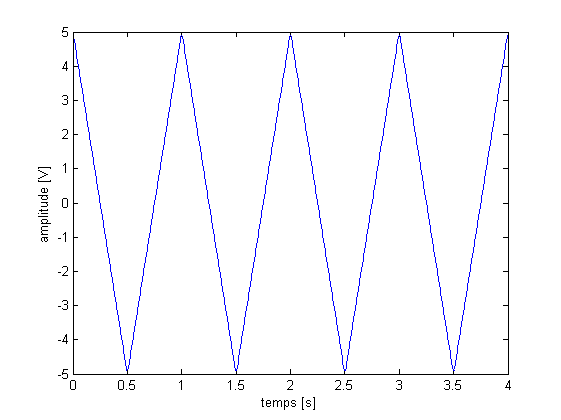
\includegraphics[scale=0.6]{img/q1-fourier-19.png}
	\caption{Décomposition en série de Fourier pour $k=1\dots19$.}
	\label{fig:q1-fourier-19}
\end{figure}

Passons maintenant au cas général, c'est à
dire avec une origine des temps quelconque.
La série doit maintenant s'écrire sous la
forme
\begin{equation}
	u(t) = \sum_{k=-\infty}^\infty C_k e^{jk\omega t}.
	\label{eq:fourier-complex}
\end{equation}
Il s'agit ensuite d'exprimer $C_k$ en fonction
de $A_k$ et $B_k$ et de trouver une expression
simple pour $C_k$ faisant usage d'exponentielles
complexes. Pour ce faire, on utilise les relations
suivantes
\[ \cos(k\omega t) = \frac{e^{jk\omega t}+e^{-jk\omega t}}{2},\]
\[ \sin(k\omega t) = \frac{e^{jk\omega t}-e^{-jk\omega t}}{2j}\]
dans l'équation \ref{eq:fourier-real}
\[ u(t) = A_0 + \sum_{k=1}^{\infty} A_k\left(\frac{e^{jk\omega t}+e^{-jk\omega t}}{2}\right)
	+ \sum_{k=1}^{\infty} B_k\left(\frac{e^{jk\omega t}-e^{-jk\omega t}}{2j}\right). \]
On met un peu d'ordre dans cette expresion et on l'égalise 
ensuite à l'équation \ref{eq:fourier-complex}
\[ A_0 + \sum_{k=1}^{\infty} \frac{(A_k-jB_k)}{2}e^{jk\omega t}
	+ \sum_{k=1}^{\infty} \frac{(A_k+jB_k)}{2}e^{-jk\omega t} = 
	\sum_{k=-\infty}^\infty C_k e^{jk\omega t}.\]
De cette égalité, on retire
\[ C_k =
	\left\{
		\begin{array}{cl}
			A_0 & \text{ pour } k = 0 \\
			\frac{(A_k-jB_k)}{2} & \text{ pour } k = 1,2,3,\dots \\
			\frac{(A_{-k}+jB_{-k})}{2} & \text{ pour } k = -1,-2,-3,\dots
		\end{array}
	\right.
\]
En sachant que $A_0$, $A_k$ et $B_k$ sont
donnés respectivement par les équations
\ref{eq:fourier-constant}, \ref{eq:fourier-coef-cos}
et \ref{eq:fourier-coef-sin}, on pour calculer
$C_k$ dans les trois cas. On montre facilement que
\[ C_k = \frac{1}{T} \int_0^T u(t)e^{-jk\omega t}\dif t\]
dans les trois cas. Cette façon de procéder est tirée de 
\cite{complex-fourier-series}.
Il ne nous reste plus maintenant qu'à prouver
que $C_{-k} = C_k^*$ dans le cas d'un signal réel,
c'est à dire $u(t) \in \R$. On trouve très facilement que
\begin{equation}
	C_{-k} = \frac{1}{T} \int_0^T u(t)e^{jk\omega t}\dif t.
	\label{eq:c-minus}
\end{equation}
Il reste à calculer $C^*_k$. En utilisant les propriétés
du complexe conjugués et en sachant que $u(t) \in \R$,
on a successivement

\[\arraycolsep=1.4pt\def\arraystretch{2.2}
	\begin{array}{cl}
		C_k^* &= 1/T \left(\int_0^T u(t)e^{-jk\omega t} \dif t\right)^* \\ 
					&= 1/T \int_0^T \left(u(t)e^{-jk\omega t}\right)^* \dif t \\
					&= 1/T \int_0^T (u(t))^*(e^{-jk\omega t})^* \dif t \\
					&= 1/T \int_0^T u(t)e^{jk\omega t} \dif t.
	\end{array}
\]

Cette expression est effectivement égale à
l'équation \ref{eq:c-minus}.

\section{Transformation non-linéaire}
%On considère pour cette question le système
%représenté à la figure \ref{fig:system}.

% Useless si je n'arrive pas à indiquer les entrées/sorties.
% En plus j'ai vraiment fait ça n'importe comment... A faire
% plus proprement la prochaine fois.
%\begin{figure}[!htb]
	%\centering
	%\begin{circuitikz}[american]
	  %\coordinate (device) at (4,0);
		%\begin{scope}[every node/.style={draw,thick, fill=	white, rectangle,text width=3cm, minimum height=2cm, text badly centered}]
        %\node[name=device] at (device) {Système non-linéaire};
    %\end{scope}
		%\draw
			%(5.65,0.7) -- (7.5,0.7)
			%(7.5,0.7) node[ocirc] (C) {}
			%(5.65,-0.7) -- (7.5,-0.7)
			%(7.5,-0.7) node[ocirc] (D) {}
			%(0.54,0.7) -- (2.39,0.7)
			%(0.54,0.7) node[ocirc] (A) {}
			%(0.54,-0.7) -- (2.39,-0.7)
			%(0.54,-0.7) node[ocirc] (B) {}
		%;
	%\end{circuitikz}
	%\caption{Système non-linéaire.}
	%\label{fig:system}
%\end{figure}
On considère pour cette question un système non-linéaire
dont le signal d'entrée est donné par $x$ et la sortie
par $h(x)$.
Dans notre cas, le signal d'entrée $x$ est $u(t)$,
le signal triangulaire de la question précédente et
$h(x)$ est une transformation non-linéaire donnée par
son développement de Taylor jusqu'à l'ordre 3 :
$h(x) \approx a+bx+cx^2+dx^3$.
Comme annoncé, les ordres 0 et 1 s'obtiennent trivialement.
L'odre 2 en revanche nécessite un peu plus de manipulation.
Repartons de l'équation \ref{eq:fourier-real}, que l'on
élève au carré
\[\arraycolsep=1.4pt\def\arraystretch{2.2}
	\begin{array}{cl}
		 u^2(t)	&= A_0^2 + \left(\sum\limits_{k=1}^\infty A_k\cos(k\omega t)\right)^2 + \left(\sum\limits_{k=1}^\infty B_k\sin(k\omega t)\right)^2\\ 
						&+~ 2A_0\sum\limits_{k=1}^\infty A_k\cos(k\omega t) + 2A_0\sum\limits_{k=1}^\infty B_k\sin(k\omega t)
						+ 2\sum\limits_{k=1}^\infty A_k\cos(\omega t)\sum\limits_{k=1}^{\infty}B_k\sin(k\omega t). 
	\end{array}
\]

On peut mettre un peu d'ordre en utilisant des doubles
sommes sur des paires d'indices $(k_1,k_2)$
\[\arraycolsep=1.4pt\def\arraystretch{2.2}
	\begin{array}{cl}
		 u^2(t)	&= A_0^2 + \sum\limits_{k_1=1}^\infty\sum\limits_{k_2=1}^\infty A_{k_1}A_{k_2}\cos(k_1\omega t)\cos(k_2\omega t) 
							+ \sum\limits_{k_1=1}^\infty\sum\limits_{k_2=1}^\infty B_{k_1}B_{k_2}\sin(k_1\omega t)\sin(k_2\omega t)\\ 
						&+~ 2A_0\sum\limits_{k_1=1}^\infty A_{k_1}\cos(k_1\omega t) + 2A_0\sum\limits_{k_1=1}^\infty B_{k_1}\sin(k_2\omega t)
						+ 2\sum\limits_{k_1=1}^\infty\sum\limits_{k_2=1}^\infty A_{k_1}B_{k_2}\cos(k_1\omega t)\sin(k_2\omega t). 
	\end{array}
\]
On utilise ensuite les formules trigonométriques qui
permettent de transformer un produit de fonctions
sinusoïdales en une somme de fonctions sinusoïdales
\[\arraycolsep=1.4pt\def\arraystretch{2.2}
	\begin{array}{cl}
		 u^2(t)	&= A_0^2 + \frac{1}{2}\sum\limits_{k_1=1}^\infty\sum\limits_{k_2=1}^\infty A_{k_1}A_{k_2}\cos\left((k_1-k_2)\omega t\right) 
						+ \frac{1}{2}\sum\limits_{k_1=1}^\infty\sum\limits_{k_2=1}^\infty A_{k_1}A_{k_2}\cos\left((k_1+k_2)\omega t\right)\\ 
						&+~ \frac{1}{2}\sum\limits_{k_1=1}^\infty\sum\limits_{k_2=1}^\infty B_{k_1}B_{k_2}\cos\left((k_1-k_2)\omega t\right)
						- \frac{1}{2}\sum\limits_{k_1=1}^\infty\sum\limits_{k_2=1}^\infty B_{k_1}B_{k_2}\cos\left((k_1+k_2)\omega t\right)\\
						&+~ \frac{1}{2}\sum\limits_{k_1=1}^\infty\sum\limits_{k_2=1}^\infty A_{k_1}B_{k_2}\sin\left((k_1+k_2)\omega t\right)
						+ \frac{1}{2}\sum\limits_{k_1=1}^\infty\sum\limits_{k_2=1}^\infty A_{k_1}B_{k_2}\sin\left((k_2-k_1)\omega t\right)\\
						&+~ 2A_0\sum\limits_{k_1=1}^\infty A_{k_1}\cos(k_1\omega t) + 2A_0\sum\limits_{k_1=1}^\infty B_{k_1}\sin(k_1\omega t).
	\end{array}
\]
Enfin, en mettant en évidence, $u^2(t)$ devient
\[\arraycolsep=1.4pt\def\arraystretch{2.2}
	\begin{array}{cl}
		 u^2(t)	&= A^2_0 + \frac{1}{2}\sum\limits_{k_1=1}^\infty\sum\limits_{k_2=1}^\infty (A_{k_1}A_{k_2}+B_{k_1}B_{k_2})\cos((k_1-k_2)\omega t) \\
						&+~ \frac{1}{2}\sum\limits_{k_1=1}^\infty\sum\limits_{k_2=1}^\infty (A_{k_1}A_{k_2}-B_{k_1}B_{k_2})\cos((k_1+k_2)\omega t) \\
						&+~ \frac{1}{2}\sum\limits_{k_1=1}^\infty\sum\limits_{k_2=1}^\infty A_{k_1}B_{k_2}(\sin\left((k_1+k_2)\omega t\right)
						+\sin\left((k_2-k_1)\omega t\right))\\
						&+~ 2A_0\sum\limits_{k_1=1}^\infty A_{k_1}\cos(k_1\omega t) + B_{k_1}\sin(k_1\omega t).
	\end{array}
\]
On voit donc facilement à partir de cette dernière équation comment calculer
les coefficients de la décomposition harmonique de $u^2(t)$ à partir des
coefficients de la décomposition harmonique de $u(t)$. En considérant
maintenant le signal $u(t)$ symétrique, $u^2(t)$ se simplifie
(car $B_k = 0$ par symétrie) et devient
\[\arraycolsep=1.4pt\def\arraystretch{2.2}
	\begin{array}{cl}
		u^2(t) 	&= A^2_0 + \frac{1}{2}\sum\limits_{k_1=1}^\infty\sum\limits_{k_2=1}^\infty A_{k_1}A_{k_2}\cos((k_1-k_2)\omega t)\\
						&+~ \frac{1}{2}\sum\limits_{k_1=1}^\infty\sum\limits_{k_2=1}^\infty A_{k_1}A_{k_2}\cos((k_1+k_2)\omega t) \\
						&+~ 2A_0\sum\limits_{k_1=1}^\infty A_{k_1}\cos(k_1\omega t).
	\end{array}
\]
Si en plus, la composante continue $A_0$ du signal est nulle,
$u^2(t)$ se simplifie encore
\[ u^2(t) = \frac{1}{2}\sum\limits_{k_1=1}^\infty\sum\limits_{k_2=1}^\infty A_{k_1}A_{k_2}\cos((k_1-k_2)\omega t)
+ \frac{1}{2}\sum\limits_{k_1=1}^\infty\sum\limits_{k_2=1}^\infty A_{k_1}A_{k_2}\cos((k_1+k_2)\omega t). \]


Enfin, considérons le cas où 
\[ h(x) = \frac{x}{\sqrt{(x/s)^2+1}}.\]
En observant le graphe de $h(x)$ pour plusieurs
valeurs de $s$ (voir figure \ref{fig:non-linear-transfer}),
on observe que ce paramètre règle en fait la saturation du circuit
(on dit que le circuit sature quand la sortie n'augmente plus
même si l'entrée augmente encore). 
On prouve également facilement que
\[ \lim_{x\to\pm\infty} h(x) = s.\]

\begin{figure}[ht]
	\centering
	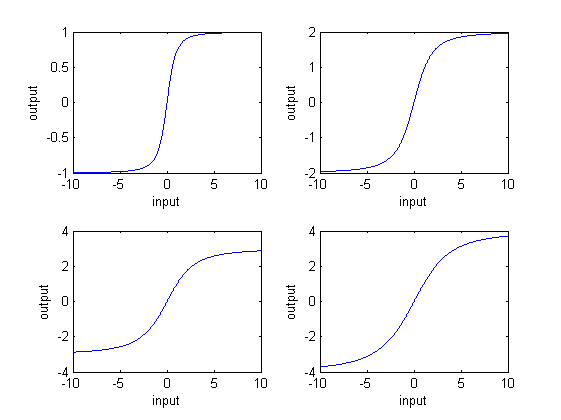
\includegraphics[scale=0.6]{img/non-linear-transfer.png}
	\caption{Graphe de la fonction $h(x)$ pour $s=1\dots4$.}
	\label{fig:non-linear-transfer}
\end{figure}

Le développement de Taylor jusqu'à l'ordre de 3 de
$h(x)$ autour de $x=0$ est donné par 
\[ h(x) \approx x-\frac{x^3}{2s^2}. \]
A l'aide de \matlab, on peut vérifier que cette
transformation non-linéaire permet effectivement
de transformer un signal triangulaire en un signal
sinusoïdal. Cette transformation est illustrée à
la figure \ref{fig:in_out_diagram}.

\begin{figure}[ht]
	\centering
	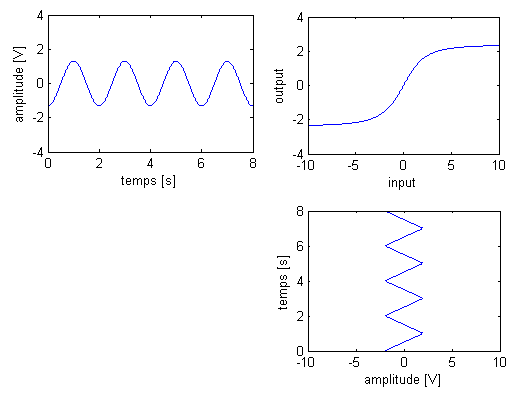
\includegraphics[scale=0.6]{img/in_out_diagram.png}
	\caption{Le signal triangulaire en entrée de la transformation
	non-linéaire $h(x)$ pour $s=2.4$ permet effectivement d'obtenir
	un signal sinusoïdal en sortie.}
	\label{fig:in_out_diagram}
\end{figure}

Cherchons maintenant un rapport $V/s$, où $V$ est
l'amplitude du signal d'entrée du système, tel que
la saturation soit ``très légère''. Pour répondre à cette question,
nous devons définir de manière plus précise ce qu'on appelle
une saturation ``très légère''. Nous avons choisis, arbitrairement
, la définition suivante : la saturation est très légère
lorsque l'amplitude de sortie vaut 95\% de l'amplitude
maximale de sortie\footnote{Nous aurions également pû choisir une définition
faisant intervenir la dérivée de $h(x)$, et indiquer que la
saturation est légère lorsque $\fdif{h}{x} \approx 0.1$ par exemple,
c'est à dire quand la pente de $h(x)$ devient faible.}.
\[ h(V) = 0.95s. \]
On trouve alors que la saturation est légère pour 
\[ \frac{V}{s} \approx 3. \]
Il est toutefois important de noter que ce rapport
dépend de la définition de saturation ``légère'' choisie.
\biblio{problem1}
\end{document}